% Source: graduate-coursework/Research/Intro_to_Agents/handouts/Part4_Planning_Workflow.tex

\documentclass[border=4pt]{standalone}
\usepackage{graphicx}
\usepackage{tikz}
\usepackage{xcolor}
\usetikzlibrary{shapes.geometric, arrows.meta, positioning, calc, fit, backgrounds}

\definecolor{UofSCGarnet}{HTML}{73000A}
\definecolor{UofSCBlack}{HTML}{000000}
\definecolor{UofSCWhite}{HTML}{FFFFFF}
\definecolor{UofSCAtlantic}{HTML}{466A9F}
\definecolor{UofSCCongaree}{HTML}{1F414D}
\definecolor{UofSCHorseshoe}{HTML}{65780B}
\definecolor{UofSCRose}{HTML}{CC2E40}
\definecolor{UofSCDarkGarnet}{HTML}{570008}
\definecolor{UofSC90Black}{HTML}{363636}
\definecolor{UofSC70Black}{HTML}{5C5C5C}
\definecolor{UofSC50Black}{HTML}{A2A2A2}

\tikzset{
    box/.style={
        draw=UofSCBlack,
        fill=#1,
        minimum width=2.5cm,
        minimum height=0.8cm,
        text=UofSCWhite,
        font=\small\bfseries,
        align=center,
        inner sep=4pt
    },
    box/.default=UofSCGarnet,
    lightbox/.style={
        draw=UofSCBlack,
        fill=UofSCWhite,
        minimum width=2.5cm,
        minimum height=0.8cm,
        text=UofSCBlack,
        font=\small,
        align=center,
        inner sep=4pt
    },
    arrow/.style={
        ->,
        >=Stealth,
        thick,
        UofSCBlack
    },
    bigarrow/.style={
        ->,
        >=Stealth,
        line width=1.5pt,
        UofSCGarnet
    },
    phase/.style={
        draw=UofSCBlack,
        fill=#1,
        minimum width=3cm,
        minimum height=1cm,
        text=UofSCWhite,
        font=\bfseries,
        align=center
    },
    phase/.default=UofSCGarnet,
    subphase/.style={
        draw=UofSC70Black,
        fill=UofSCWhite,
        minimum width=2.8cm,
        minimum height=0.6cm,
        text=UofSCBlack,
        font=\scriptsize,
        align=center
    },
    cyclebox/.style={
        draw=UofSCBlack,
        line width=1.5pt,
        fill=#1,
        minimum width=2cm,
        minimum height=1.2cm,
        text=UofSCWhite,
        font=\bfseries,
        align=center
    },
    cyclebox/.default=UofSCGarnet
}

\begin{document}
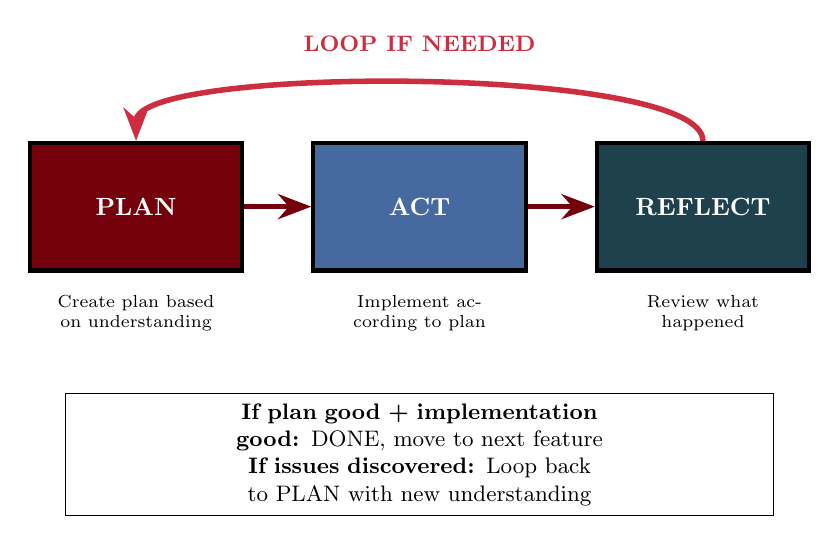
\begin{tikzpicture}[scale=0.9, transform shape]
        % Plan box
        \node[cyclebox=UofSCGarnet, minimum width=3cm, minimum height=1.8cm] (plan) at (-4,0) {PLAN};
        \node[font=\scriptsize, text width=2.8cm, align=center] at (-4,-1.5) {Create plan based on understanding};

        % Act box
        \node[cyclebox=UofSCAtlantic, minimum width=3cm, minimum height=1.8cm] (act) at (0,0) {ACT};
        \node[font=\scriptsize, text width=2.8cm, align=center] at (0,-1.5) {Implement according to plan};

        % Reflect box
        \node[cyclebox=UofSCCongaree, minimum width=3cm, minimum height=1.8cm] (reflect) at (4,0) {REFLECT};
        \node[font=\scriptsize, text width=2.8cm, align=center] at (4,-1.5) {Review what happened};

        % Arrows
        \draw[bigarrow, line width=2pt] (plan) -- (act);
        \draw[bigarrow, line width=2pt] (act) -- (reflect);
        \draw[bigarrow, line width=2pt, UofSCRose] (reflect.north) .. controls (4,2) and (-4,2) .. (plan.north);

        % Loop back label
        \node[text=UofSCRose, font=\small\bfseries] at (0,2.3) {LOOP IF NEEDED};

        % Decision box
        \node[lightbox, minimum width=10cm, minimum height=1.5cm, text width=9.5cm] at (0,-3.5) {
            \textbf{If plan good + implementation good:} DONE, move to next feature\\
            \textbf{If issues discovered:} Loop back to PLAN with new understanding
        };
    \end{tikzpicture}
\end{document}
